\chapter{Additional data and tables}\label{app:A}
\section{Functional requirements}\vspace{0.3cm}
   \resizebox{\textwidth}{!}{%
    \begin{tabular} {|p{5cm}|c|p{7cm}|} %\begin{tabular}{|p{2cm}|p{5cm}|}  
    \hline
    What to \hypertarget{thistable}{do}? & User Story  \\
    \hline
    Login on mobile & As a new user, I want to sign up using my existing Google account so that I don't have to keep track of another account. \\
    \hline
    Functions for teacher & As a teacher, I want to create classes, add students to them, and assign them tasks/projects.\\
    \hline
    List of tasks/projects & As an existing student, I want to see all my tasks, so that I don't miss any of them. \\
    \hline
    Function for breaking down tasks & As a student, I want to break down assigned tasks, and prioritize them, so that I could work effectively. \\
    \hline
    View statistics & As a teacher, I want to see statistics on plagiarism, to make sure that evaluating process is fare. \\
    \hline
    Progress Tracking block & As a teacher, I want to see students' progress for specific data range. \\
    \hline
    Add timer page & As a student, I want to see time I spent on particular task, so that I can manage my energy and distribute my time wisely.\\
    \hline
    
    \end{tabular}
    }
\section{Images}
\hypertarget{thisimage}{Similarity measuring using python:}\newline
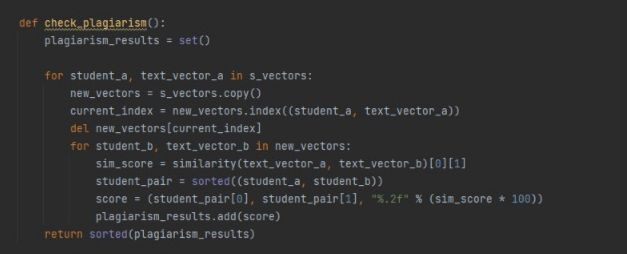
\includegraphics{code1.jpeg}
